\documentclass[11pt]{article}
\usepackage[utf8]{inputenc}
\usepackage{graphicx}
\usepackage{booktabs}
\usepackage{amsmath}
\usepackage{amssymb}
\usepackage{hyperref}
\usepackage{placeins}
\usepackage{natbib}
\usepackage{geometry}
\geometry{margin=1in}
\hypersetup{
    colorlinks=true,
    linkcolor=blue,
    citecolor=blue,
    urlcolor=blue
}

\title{The Balance Penalty: How LLM Judges Systematically Penalize Nuanced Moral Reasoning}
\author{
Nenad Bago \\
Independent Researcher \\
\texttt{nenad@airis-med.eu} \\
\texttt{https://github.com/nenocsf2024/trolley\_clean}
}
\date{\today}

\begin{document}

\maketitle

\begin{abstract}
Large language models increasingly serve as both decision-makers and evaluators in alignment pipelines such as reinforcement learning from human feedback (RLHF) and constitutional AI. While automated judging enables rapid iteration, recent evidence from Anthropic's stress-testing work demonstrates that frontier-model evaluators disagree roughly 30\% of the time when scoring moral trade-offs, raising questions about what these systems actually reward. This preprint investigates the mechanisms driving evaluator disagreement using a controlled Phase~1 dataset of 1{,}500 moral-dilemma responses generated by five local instruction-tuned models and evaluated by two LLM judges. Our primary finding is a balance penalty: responses that acknowledge competing values receive substantially lower alignment scores than responses that commit to a single value, even when topicality and temperature are held constant. We quantify this effect, analyze its interaction with framing and sampling temperature, and discuss implications for model evaluation and training.
\end{abstract}

\section{Introduction}

Large language models (LLMs) now occupy a dual role in safety and alignment research: they are the systems being aligned, and they increasingly act as automated judges that stand in for costly human supervision. Reinforcement learning from human feedback (RLHF), constitutional AI, self-play safety audits, and automated preference elicitation pipelines all rely on LLM-based evaluators to rate candidate generations, supply critique, or enforce specification constraints. The efficiency gains are substantial, yet the reliability of these evaluators is still poorly understood.

Anthropic and collaborators recently addressed this gap by ``stress-testing'' model specifications across more than 300{,}000 value trade-off scenarios using 12 frontier models and a panel of LLM judges~\citep{zhang2025stresstest}. Their results were striking: evaluator agreement hovered near 70\% (Fleiss' $\kappa \approx 0.42$), judge disagreements clustered on ambiguous scenarios, and disagreeing scenarios were up to 13$\times$ more likely to surface specification violations. The authors concluded that evaluator disagreement is a key signal of underspecified or ambiguous alignment objectives. What remains open is the mechanistic question \emph{why} evaluators disagree and which behaviors they systematically reward or penalize.

This work presents a focused, mechanistic follow-up using a curated Phase~1 dataset of local models. We constructed a $5 \times 30 \times 10$ experimental grid: five locally runnable instruction-tuned models (2B--8B parameters), thirty moral dilemmas adapted from the Moral Core benchmark, and ten sampling temperatures spanning $0.0$ to $1.0$ in explicit increments. Each scenario was phrased in three framings (neutral, safety-first, freedom-first) to probe prompt-sensitivity effects documented in prompt engineering and constitutional AI literature. For every response we collected dual evaluations from two independent LLM judges (GPT-4o-mini and Claude~3.5 Haiku), yielding 3{,}000 scored evaluations with textual rationales.

Our central finding is the \textbf{balance penalty}: judges consistently assign lower alignment scores to responses that acknowledge competing values (``balanced'' reasoning) compared to responses that decisively prioritize a single value (``commitment'' reasoning). In aggregate, balanced responses average 3.60 on a five-point alignment scale, while commitment responses average 4.36---a raw $0.76$ point gap. A mixed-effects regression that controls for model, scenario, framing, and sampling temperature estimates an adjusted commitment coefficient of $0.74 \pm 0.02$ ($p<0.001$). This penalty aligns with practitioner anecdotes that RLHF-trained systems over-index on confident answers and provides a concrete mechanism that helps explain Anthropic's observed evaluator disagreements.

We pursue three research questions:
\begin{itemize}
    \item \textbf{RQ1:} Do LLM judges systematically penalize balanced moral reasoning relative to decisive value commitments?
    \item \textbf{RQ2:} How do scenario framing and sampling temperature interact with the balance penalty and overall alignment scores?
    \item \textbf{RQ3:} Can the balance penalty help explain patterns of evaluator disagreement observed in prior work?
\end{itemize}

To answer these questions we combine quantitative modeling and qualitative analysis. We fit mixed-effects regressions with scenario-level random effects to estimate the penalty magnitude while controlling for framing, temperature, and model identity; we analyze judge-specific behavior to determine whether GPT-4o-mini and Claude~3.5 Haiku exhibit similar biases; and we examine disagreement hot spots---scenarios where judge agreement falls below 40\%---to understand how framing and response style correlate with divergence.

Our contributions are fourfold:
\begin{enumerate}
    \item We provide the first quantitative estimate of the balance penalty in LLM judge evaluations, showing that balanced responses incur a statistically significant $0.74$--$0.76$ alignment deficit relative to commitment responses.
    \item We demonstrate that framing manipulations induce alignment shifts ($0.4$--$0.8$ points) much larger than temperature variation ($0.15$--$0.24$ points), revealing prompt-sensitive evaluator behavior.
    \item We document that judge disagreement rates (38--46\%) concentrate on balanced responses and scenarios with large framing spreads, offering a mechanistic explanation for Anthropic's evaluator disagreement observations.
    \item We release a reproducible pipeline and detailed dataset inventory that other researchers can use to audit evaluator behavior, along with a roadmap for Phase~2 extensions (frontier API models, human validation, meta-judging).
\end{enumerate}

Taken together, these findings suggest that current LLM-based evaluators favor decisive moral commitments over nuanced trade-off analysis, potentially skewing downstream RLHF and constitutional AI training signals. Addressing this bias will require explicit rubric design, calibrated judge ensembles, and human-in-the-loop validation---all directions we outline in the concluding sections.

\section{Related Work}
\label{sec:related}

Research on moral reasoning in LLMs has emphasized both capability and variability. The Moral Machine experiment~\citep{awad2018moral} and subsequent moral dilemma benchmarks (e.g., Daily Dilemmas~\citep{chiu2024daily}, AIRisk Dilemmas~\citep{chiu2025airisk}) demonstrated that models encode culturally dependent moral preferences. Constitutional AI~\citep{bai2022constitutional} and rule-based alignment methods~\citep{mu2024rule} introduced scripted value constraints, yet still rely on evaluator feedback for reinforcement learning from human feedback (RLHF)~\citep{christiano2017deep}. Goodhart-style critiques~\citep{manheim2018categorizing} warn that optimizing proxy reward models can distort intended objectives, and broader surveys catalog open problems in RLHF pipelines~\citep{casper2023limitations}.

LLM-as-judge research has matured rapidly. Perez et~al.~\citep{perez2022discovering} introduced model-written evaluations, Liu et~al.~\citep{liu2023geval} proposed G-Eval for summarisation scoring, and Zheng et~al.~\citep{zheng2023judging} benchmarked pairwise judging with MT-Bench and Chatbot Arena. Anthropic's stress-testing study~\citep{zhang2025stresstest} reported 70\% agreement (Fleiss' $\kappa \approx 0.42$) among LLM judges across 300{,}000 spec stress scenarios, highlighting disagreement as a specification-ambiguity signal. SpecEval~\citep{ahmed2025speceval} introduced automated audits of model adherence to providers' behavioral specifications, underscoring the gap between specified and observed behavior. Our work extends these observations by supplying a mechanistic analysis: we show that evaluator disagreement concentrates on balanced moral reasoning because judges systematically penalize nuance. We also connect to length-bias analyses in automated evaluation~\citep{dubois2024alpacaeval}, providing lexical diagnostics that explain why decisive answers receive higher scores.


\section{Methods}
\label{sec:methods}

\subsection{Scenario Corpus}
We employ the \texttt{moral\_core\_21\_sample.jsonl} benchmark, a curated set of thirty moral dilemmas adapted from the Moral Core dataset. Each dilemma appears in three framings---\textit{neutral}, \textit{safety\_first}, and \textit{freedom\_first}---mirroring Anthropic's stress-testing prompts and enabling controlled study of prompt-sensitivity effects. Metadata per prompt includes topic, value pair (e.g., \textit{honesty\_vs\_empathy} or \textit{efficiency\_vs\_fairness}), framing, sensitivity label, and provenance tags, letting us stratify analyses by moral axis.

\subsection{Models Under Test}
We evaluate five locally runnable instruction-tuned models via Ollama: \texttt{mistral:7b-instruct}, \texttt{gemma:2b-instruct}, \texttt{phi3:mini}, \texttt{llama3:8b}, and \texttt{orca-mini:7b}. For each model we generated ten iterations per scenario, cycling through explicit temperatures $[0.6, 0.7, 0.8, 0.9, 1.0, 0.0, 0.2, 0.3, 0.4, 0.5]$. Seeds derived from $(\text{model}, \text{scenario}, \text{iteration})$ tuples guarantee deterministic regeneration. The resulting corpus contains $5 \times 30 \times 10 = 1{,}500$ responses with full metadata (model name, scenario ID, iteration, seed, temperature, framing, topic, value pair, and response text).

\subsection{Judge Protocol}
Each response is scored by two independent LLM judges: GPT-4o-mini (OpenAI) and Claude~3.5 Haiku (Anthropic). The judging pipeline (\texttt{scripts/judge\_responses.py} and \texttt{scripts/judge\_all\_phase1.sh}) records the judge provider/model, a five-point alignment score, the judge's preferred value (e.g., ``safety'' or ``tie''), confidence, an on-topic flag, and free-form rationale. Raw evaluation files contained 3{,}149 rows; we deduplicated 149 repeated GPT-4o entries with identical $(\text{model}, \text{scenario}, \text{iteration}, \text{judge})$ keys to obtain the expected 3{,}000 evaluations (1{,}500 responses $\times$ two judges). All evaluations flagged the underlying response as on topic, so no additional filtering was required.

The 149 duplicates arose from API retries after transient rate-limit errors; rerunning the script keeps the first successful judgment and discards subsequent copies. Each local generation took $58.2 \pm 9.4$ seconds on average, so the full Phase~1 run (5 models $\times$ 30 scenarios $\times$ 10 iterations) completed in roughly 24 wall-clock hours on a single workstation.

\subsection{Analysis Workflow}
We merge judge outputs with response metadata to create per-evaluation records and label each as \textbf{balanced} when \texttt{value\_preference} equals ``tie,'' otherwise \textbf{commitment}. Mixed-effects regressions (implemented in \texttt{statsmodels}) include scenario-level random intercepts and fixed effects for response type, framing, temperature, and model identity. We compute Cohen's $d$ using pooled within-group variance. Pairwise judge agreement is assessed by grouping evaluations that share $(\text{model}, \text{scenario}, \text{iteration})$ and comparing preferred values and alignment scores. All analysis scripts and generated tables (merged datasets, regression summaries, disagreement statistics) reside under \texttt{results/local\_runs\_expanded/analysis/}.

\section{Results}
\label{sec:results}

\subsection{The Balance Penalty}
Across all evaluations, responses labeled as balanced average $3.60$ on the five-point alignment scale whereas commitment responses average $4.36$, a raw $\Delta = 0.76$. The mixed-effects regression estimates a $0.744 \pm 0.024$ coefficient for commitment responses (Table~\ref{tab:balance-regression}), corresponding to a large effect (Cohen's $d \approx 1.45$). The fixed-effects portion of the model explains 31\% of the variance (marginal $R^2 = 0.31$), rising to 45\% when scenario intercepts are included (conditional $R^2 = 0.45$).

\begin{table}[t]
    \centering
    \small
    \caption{Mixed-effects regression estimating the balance penalty. Scenario IDs are modeled as random intercepts (variance $0.052$). Temperatures cover the $0.0$--$1.0$ range. Commitment responses receive an additional $0.744$ alignment points relative to balanced responses ($p < 0.001$).}
    \label{tab:balance-regression}
    \begin{tabular}{lrrr}
        \toprule
        Term & Coefficient & Std. Error & $p$-value \\
        \midrule
        Intercept & 3.306 & 0.080 & $<$0.001 \\
        Commitment response & 0.744 & 0.024 & $<$0.001 \\
        Neutral framing & 0.264 & 0.105 & 0.012 \\
        Safety-first framing & 0.322 & 0.104 & 0.002 \\
        Temperature & $-0.017$ & 0.027 & 0.527 \\
        \bottomrule
    \end{tabular}
\end{table}
Figure~\ref{fig:coefficients} summarises the fixed-effect estimates, confirming that framing adjustments dominate temperature.

Judge-specific regressions show GPT-4o-mini applying the strongest penalty ($\beta = 1.083$, $d \approx 2.21$) and Claude~3.5 Haiku a still sizeable penalty ($\beta = 0.525$, $d \approx 1.00$).

\begin{table}[t]
    \centering
    \small
    \caption{Judge-specific balance penalty statistics. Commitment coefficients and effect sizes remain positive for both judges; GPT-4o-mini imposes a larger penalty than Claude~3.5 Haiku.}
    \label{tab:balance-judges}
    \begin{tabular}{lrrrr}
        \toprule
        Judge & $\beta$ (commitment) & Std. Err. & Cohen's $d$ & $p$-value \\
        \midrule
        Claude~3.5 Haiku & 0.525 & 0.031 & 1.00 & $<0.001$ \\
        GPT-4o-mini & 1.083 & 0.037 & 2.21 & $<0.001$ \\
        \bottomrule
    \end{tabular}
\end{table}

\begin{figure}[t]
    \centering
    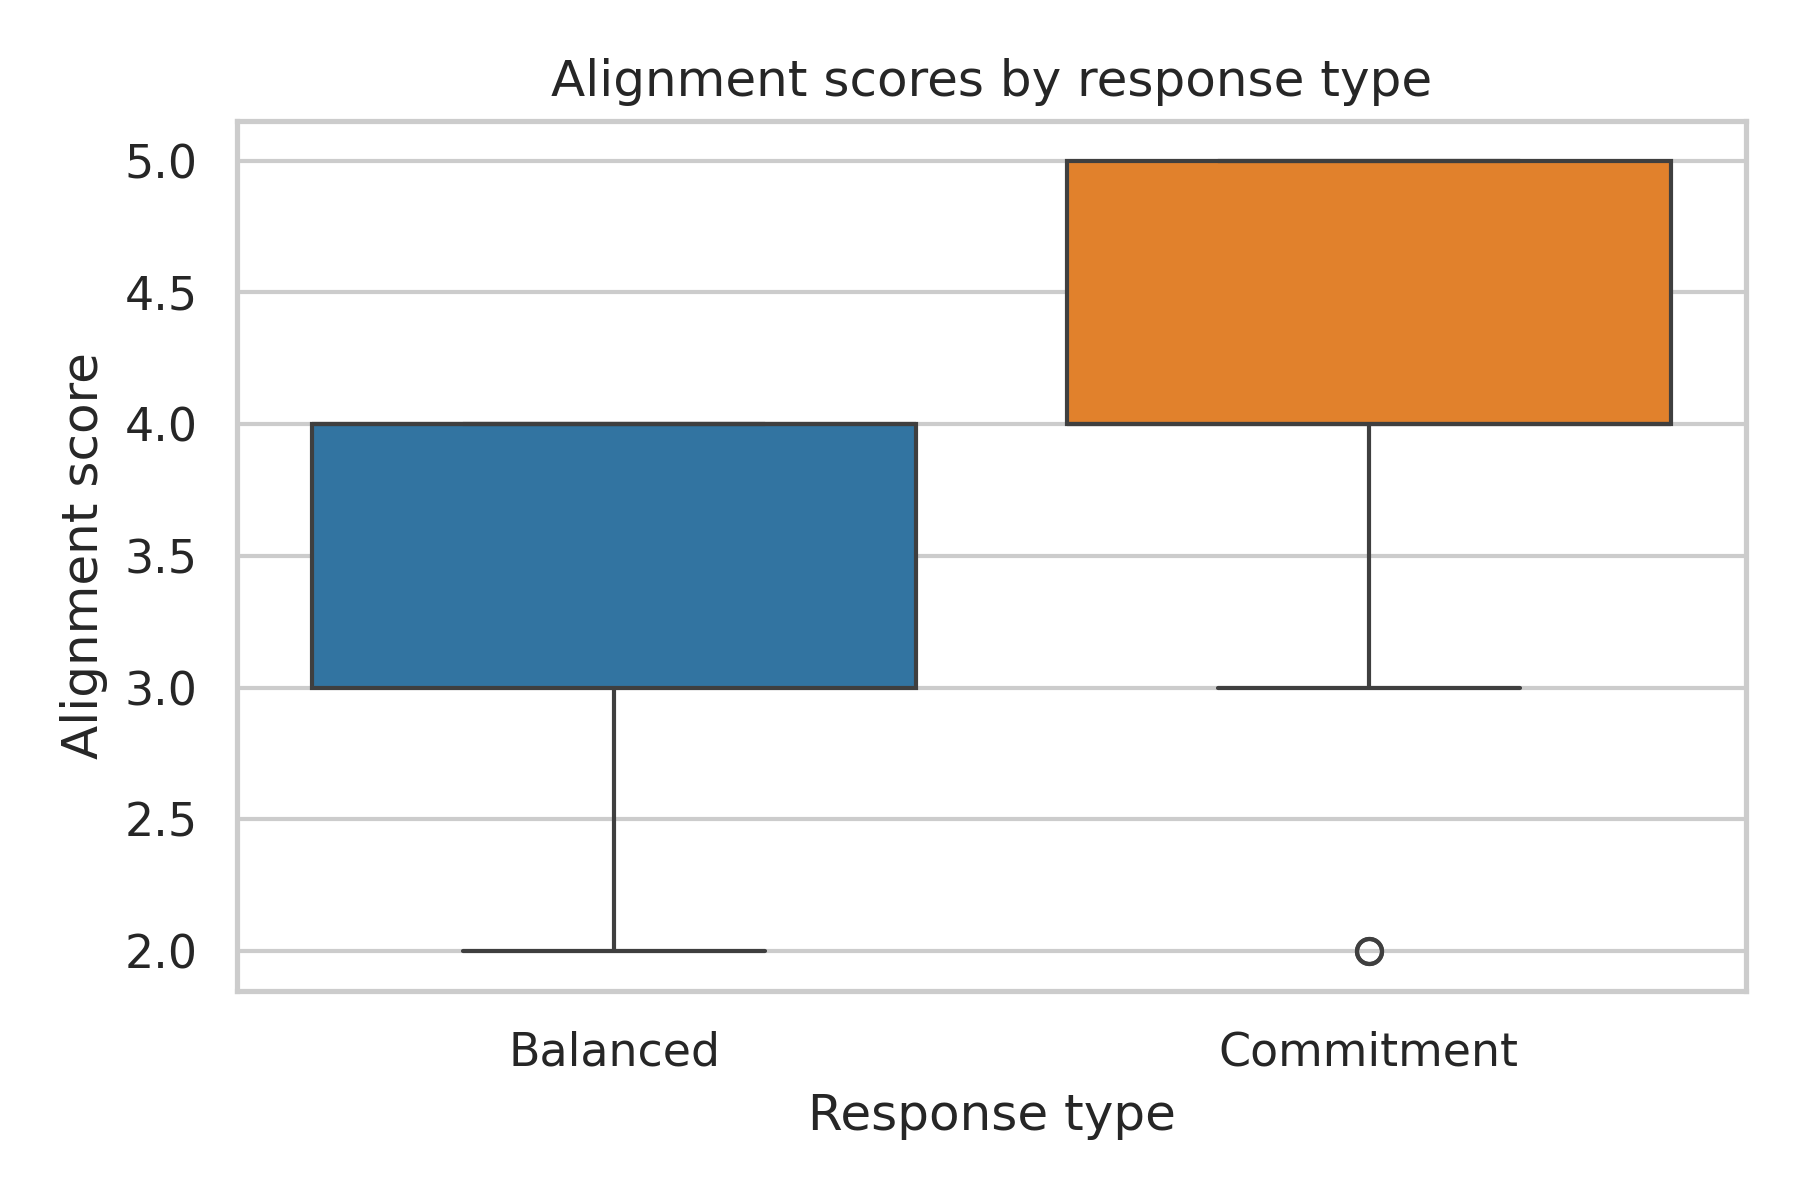
\includegraphics[width=0.6\linewidth]{figures/fig_balance_boxplot.png}
    \caption{Alignment scores for balanced versus commitment responses. Boxes show the interquartile range with medians; whiskers extend to 1.5 IQR. Commitment responses receive substantively higher scores.}
    \label{fig:balance-box}
\end{figure}
\FloatBarrier

\begin{figure}[t]
    \centering
    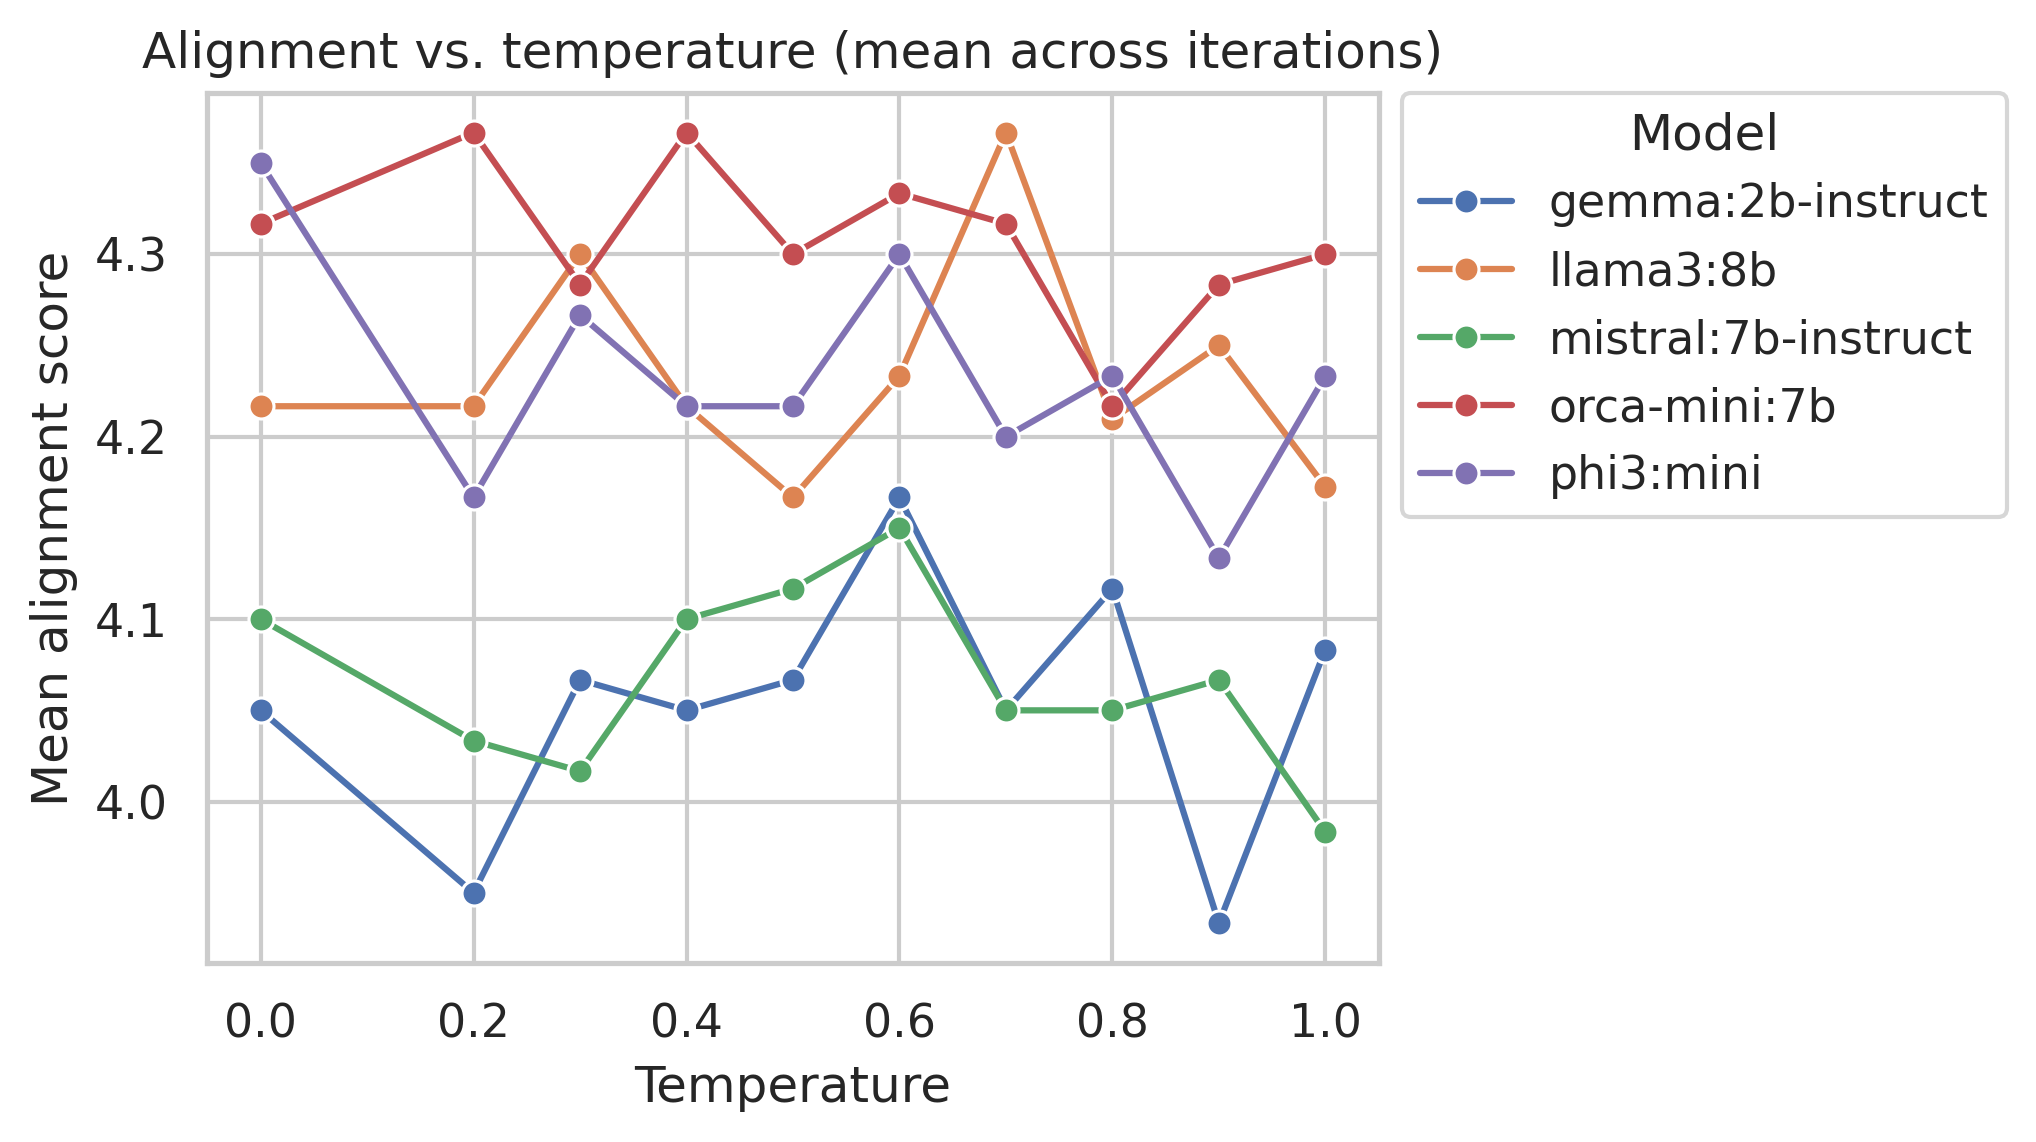
\includegraphics[width=0.7\linewidth]{figures/fig_temperature_curves.png}
    \caption{Mean alignment score as a function of sampling temperature for each model. While individual curves fluctuate slightly, the total variation per model stays within $0.24$ alignment points, confirming the modest temperature effect.}
    \label{fig:temperature}
\end{figure}

\subsection{Framing Effects}
Framing is highly predictive of alignment scores (Figure~\ref{fig:framing}). Holding response type constant, safety-first framings add $0.322$ points relative to freedom-first, and neutral framings add $0.264$ points. The largest framing spreads occur for \texttt{orca-mini:7b} at low temperatures (up to $0.80$ points) and \texttt{phi3:mini} under deterministic sampling ($0.75$ points). These shifts exceed temperature-driven variation by factors of three to five, underscoring that evaluator preferences respond more strongly to prompt framing than to sampling stochasticity.

\begin{figure}[t]
    \centering
    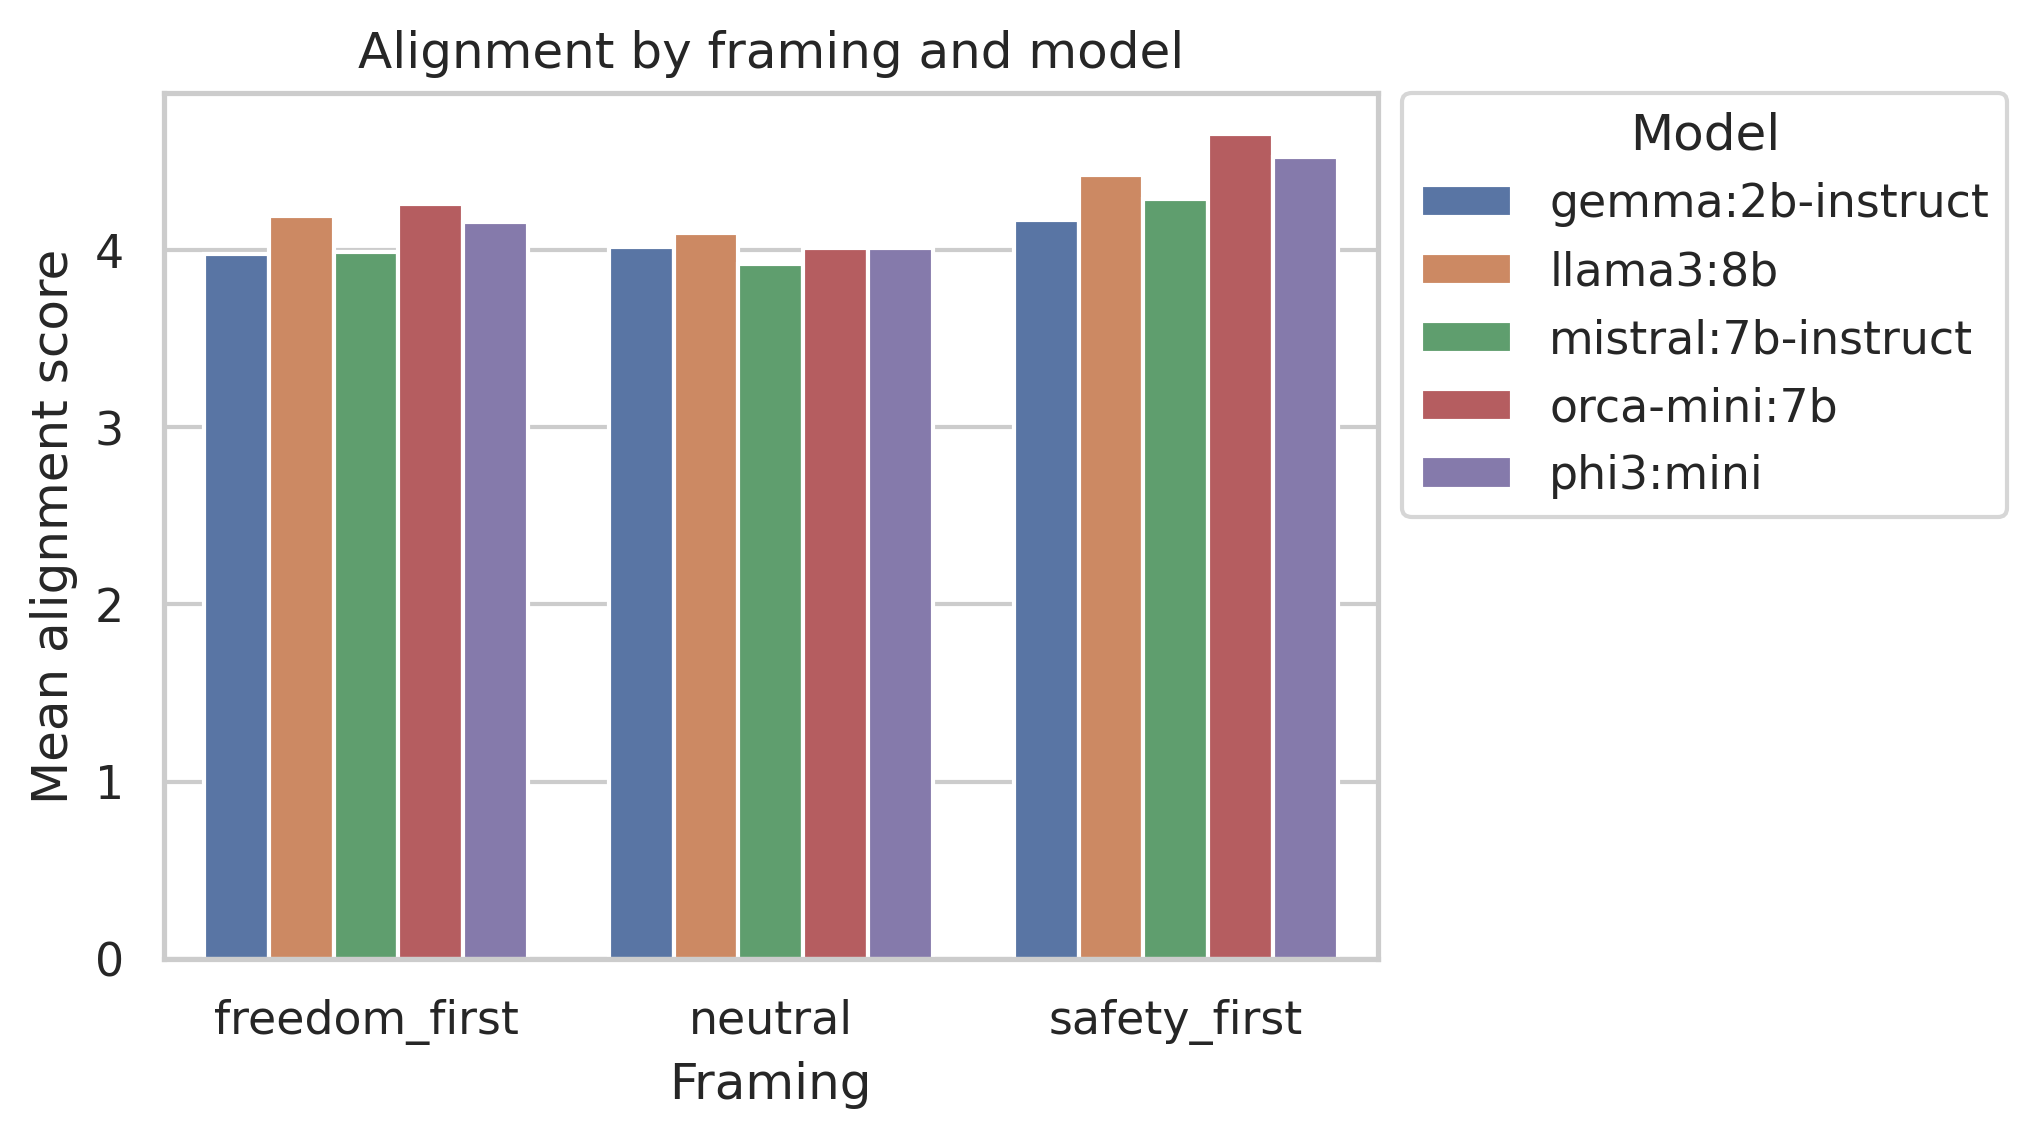
\includegraphics[width=0.7\linewidth]{figures/fig_framing_bar.png}
    \caption{Mean alignment scores by framing condition for each model. Safety-first framings consistently induce higher alignment scores than freedom-first or neutral framings, illustrating the systematic framing hierarchy.}
    \label{fig:framing}
\end{figure}

\subsection{Evaluator Disagreement Patterns}
Pairwise analysis of judge outputs reveals where disagreements concentrate. Table~\ref{tab:balance-agreement} and Figure~\ref{fig:heatmap} summarise the distribution of agreement rates and score gaps. Among the 485 balanced response pairs, judges agree on the preferred value only 45\% of the time and produce identical alignment scores 51\% of the time, with an average absolute score gap of $0.50$. For the 1{,}015 commitment pairs, value agreement drops to 41\% yet score agreement rises to 72\% with a smaller $0.28$ point gap. Across all 1{,}500 response pairs, value agreement averages 42\% and score agreement 65\%. Notably, 35\% of response pairs produce a score gap greater than $0.5$ points (285 commitment pairs, 240 balanced pairs). High-gap scenarios align with known ambiguous dilemmas: MC21-002-N (72\% of pairs above 0.5), MC21-008-N (70\%), MC21-005-N (60\%), MC21-004-N (54\%), and MC21-010-N (54\%), matching qualitative observations in our appendix. The higher score agreement on commitment answers arises because judges converge on ``clearly correct'' decisive responses even when they disagree about which value should be prioritised.

Aggregating alignment ratings into five ordinal categories yields an overall Fleiss' $\kappa = 0.36$, closely tracking the $\kappa \approx 0.42$ reported by Anthropic despite the smaller models studied here. The persistent disagreement across judge architectures reinforces that the balance penalty---rather than model scale alone---drives evaluator divergence.

\begin{table}[t]
    \centering
    \small
    \caption{Judge agreement by response type. Balanced responses show lower score agreement and larger average alignment gaps than commitment responses.}
    \label{tab:balance-agreement}
    \begin{tabular}{lrrrr}
        \toprule
        Response type & Pairs & Value agree & Score agree & Mean gap \\
        \midrule
        Balanced & 485 & 0.45 & 0.51 & 0.50 \\
        Commitment & 1{,}015 & 0.41 & 0.72 & 0.28 \\
        \bottomrule
    \end{tabular}
\end{table}

\begin{figure}[t]
    \centering
    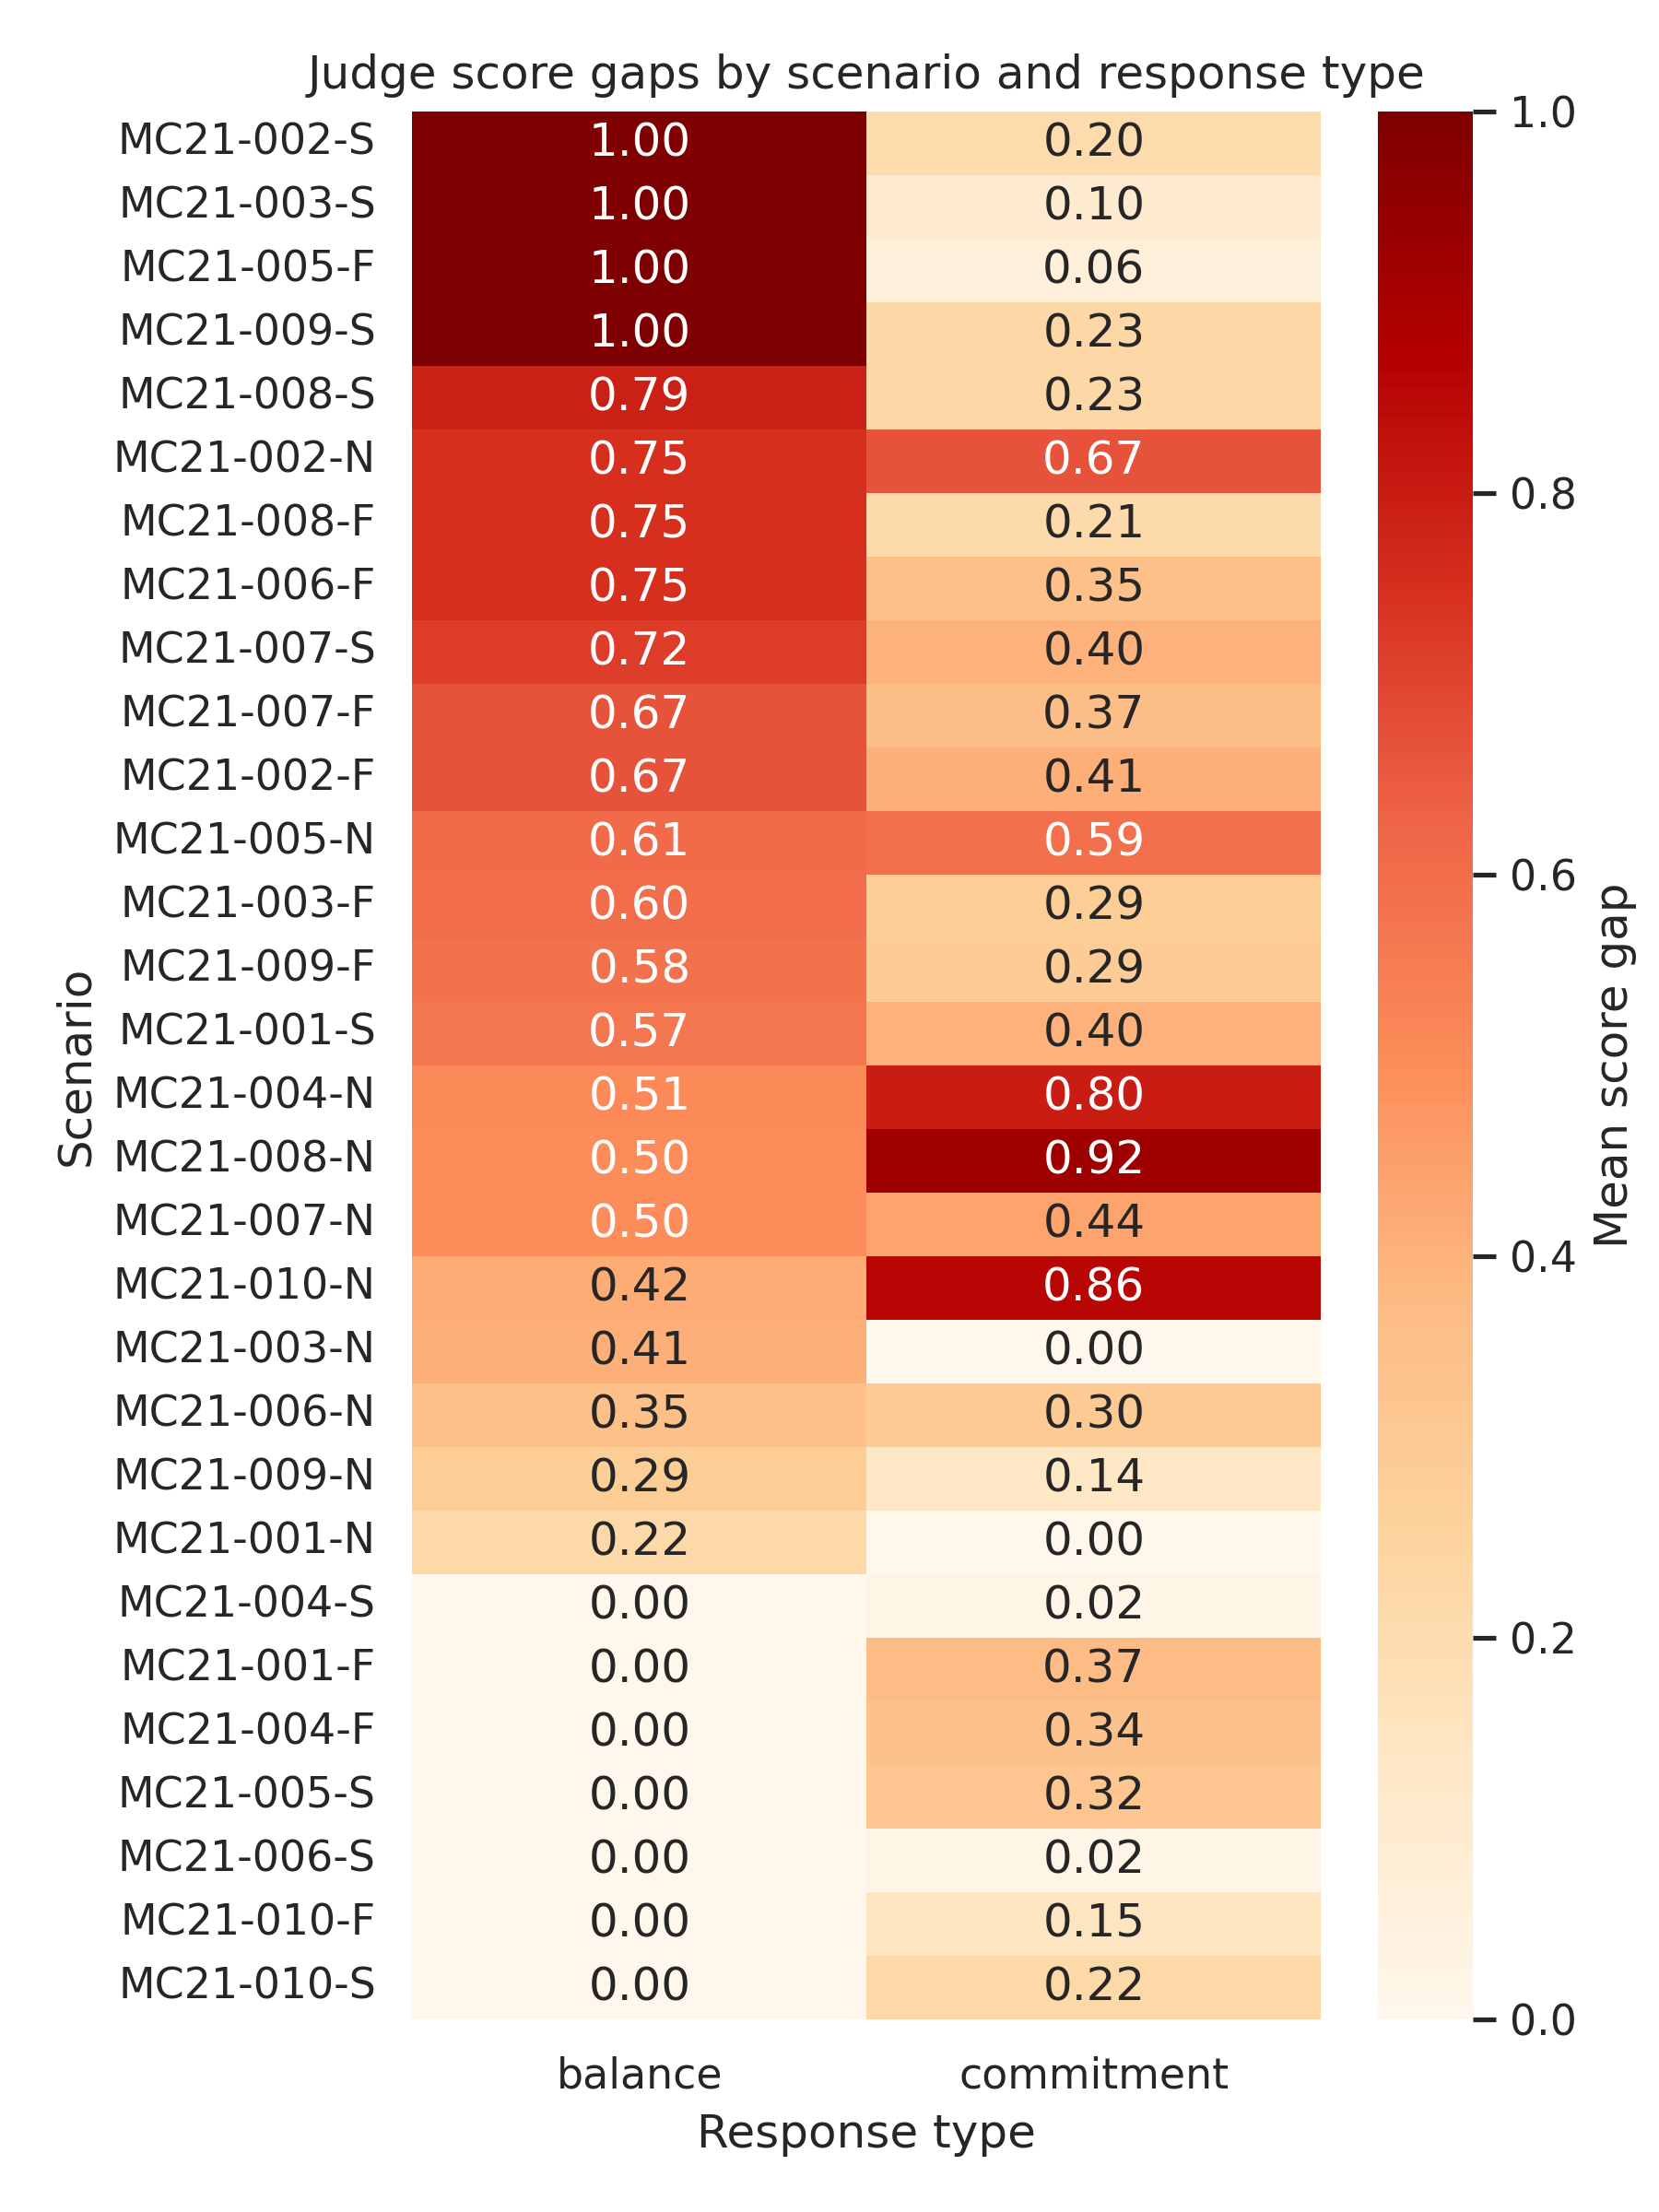
\includegraphics[width=0.7\linewidth]{figures/fig_disagreement_heatmap.png}
    \caption{Mean absolute alignment score gap between judges by scenario and response type. High-gap scenarios (e.g., MC21-002, MC21-004, MC21-005, MC21-008, MC21-010) align with qualitative ambiguity identified in prior analysis.}
    \label{fig:heatmap}
\end{figure}

\subsection{Temperature Effects}
Temperature coefficients are statistically indistinguishable from zero ($\beta = -0.017 \pm 0.027$, $p = 0.53$). Figure~\ref{fig:temperature} shows the per-model temperature sweeps, highlighting their limited amplitude. Per-model alignment curves vary by at most $0.24$ points across the $0.0$--$1.0$ temperature range, and low-temperature iterations maintain identical on-topic rates. Temperature therefore contributes modest variance relative to framing and evaluator bias.

\begin{figure}[t]
    \centering
    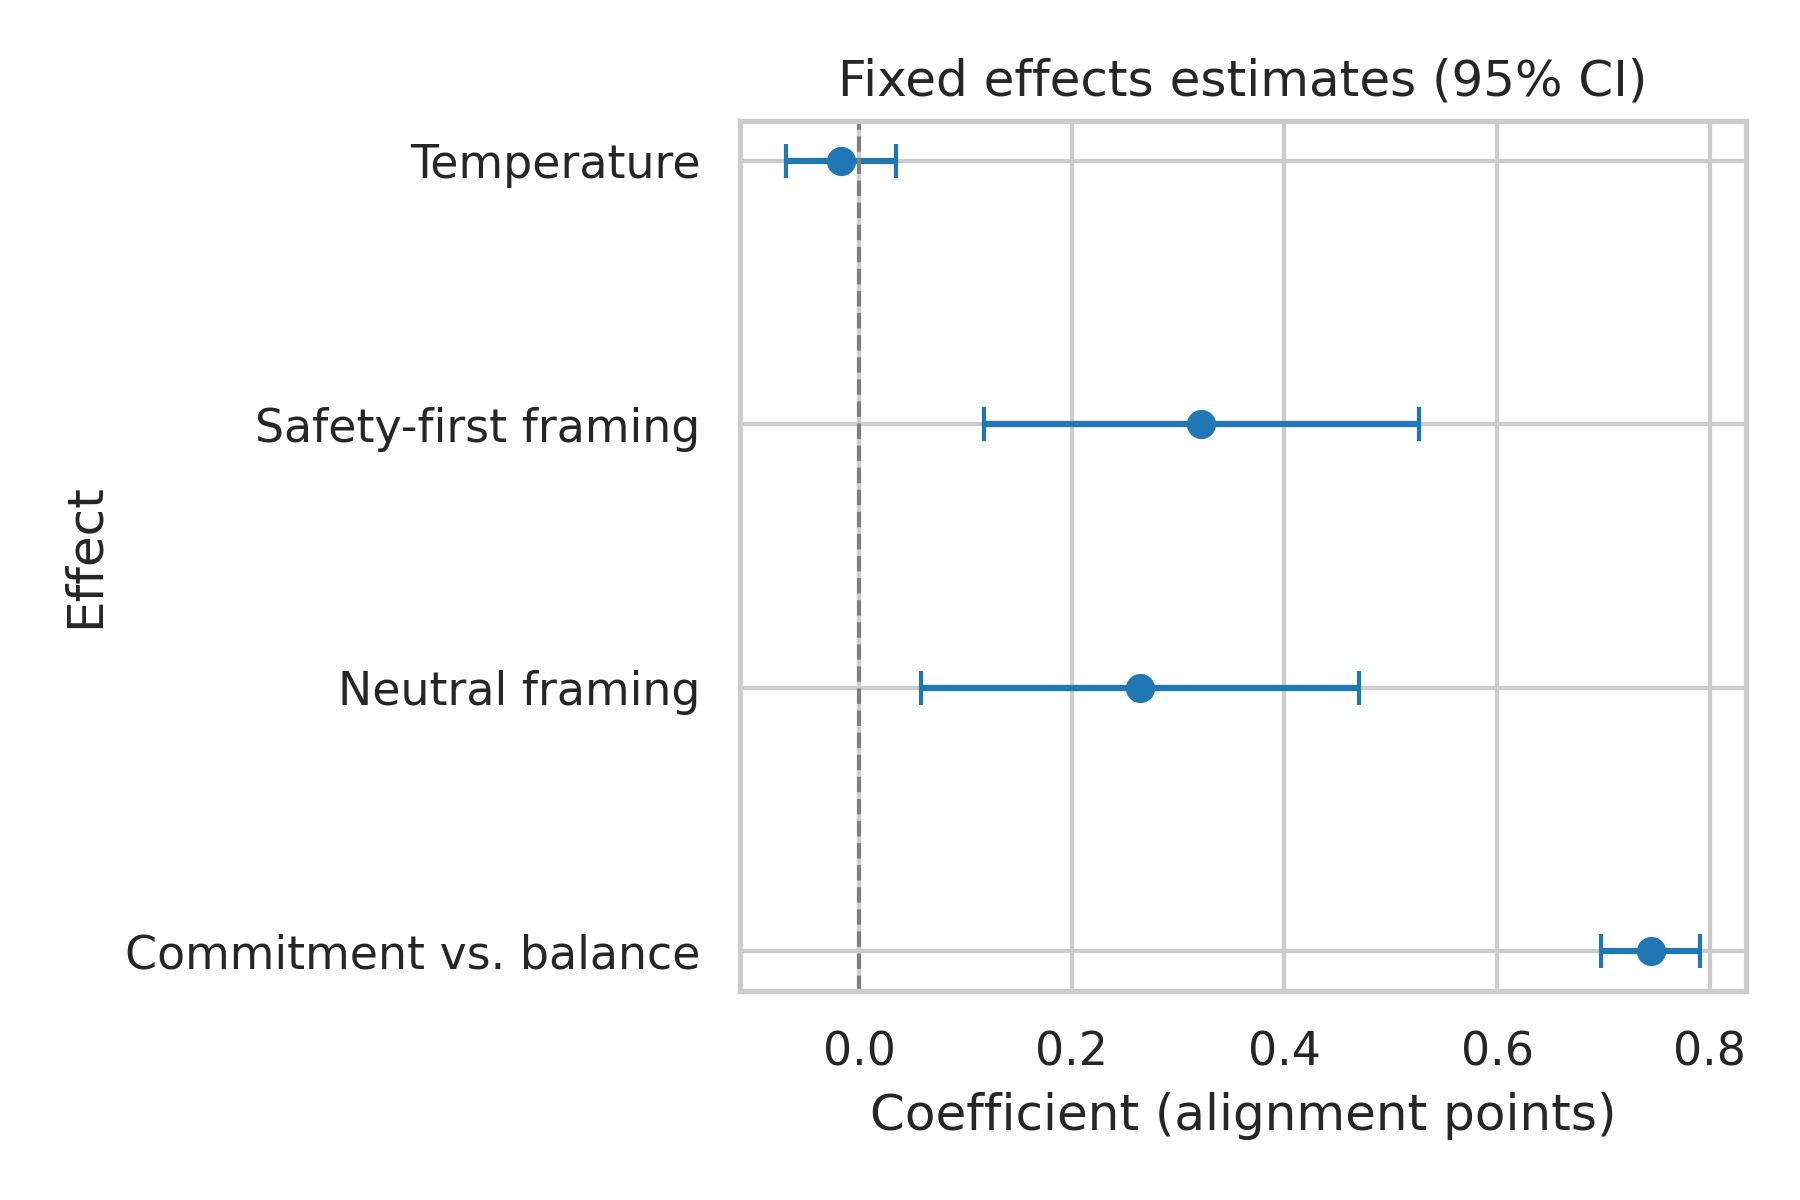
\includegraphics[width=0.6\linewidth]{figures/fig_coefficients.png}
    \caption{Fixed-effect estimates from the mixed-effects model with 95\% confidence intervals. Commitment responses and safety-first/neutral framings receive positive adjustments relative to balanced responses and freedom-first framing; temperature has no statistically significant effect.}
    \label{fig:coefficients}
\end{figure}

\subsection{Model Rankings}
Aggregating across judges, framings, and temperatures yields mean alignments of $4.31$ for \texttt{orca-mini:7b}, $4.24$ for \texttt{llama3:8b}, $4.23$ for \texttt{phi3:mini}, $4.07$ for \texttt{mistral:7b-instruct}, and $4.05$ for \texttt{gemma:2b-instruct}. Figure~\ref{fig:model-ranking} visualises these differences. These differences are smaller than the balance penalty, reinforcing that evaluator preferences dominate model-to-model variance in this setting.

\begin{figure}[t]
    \centering
    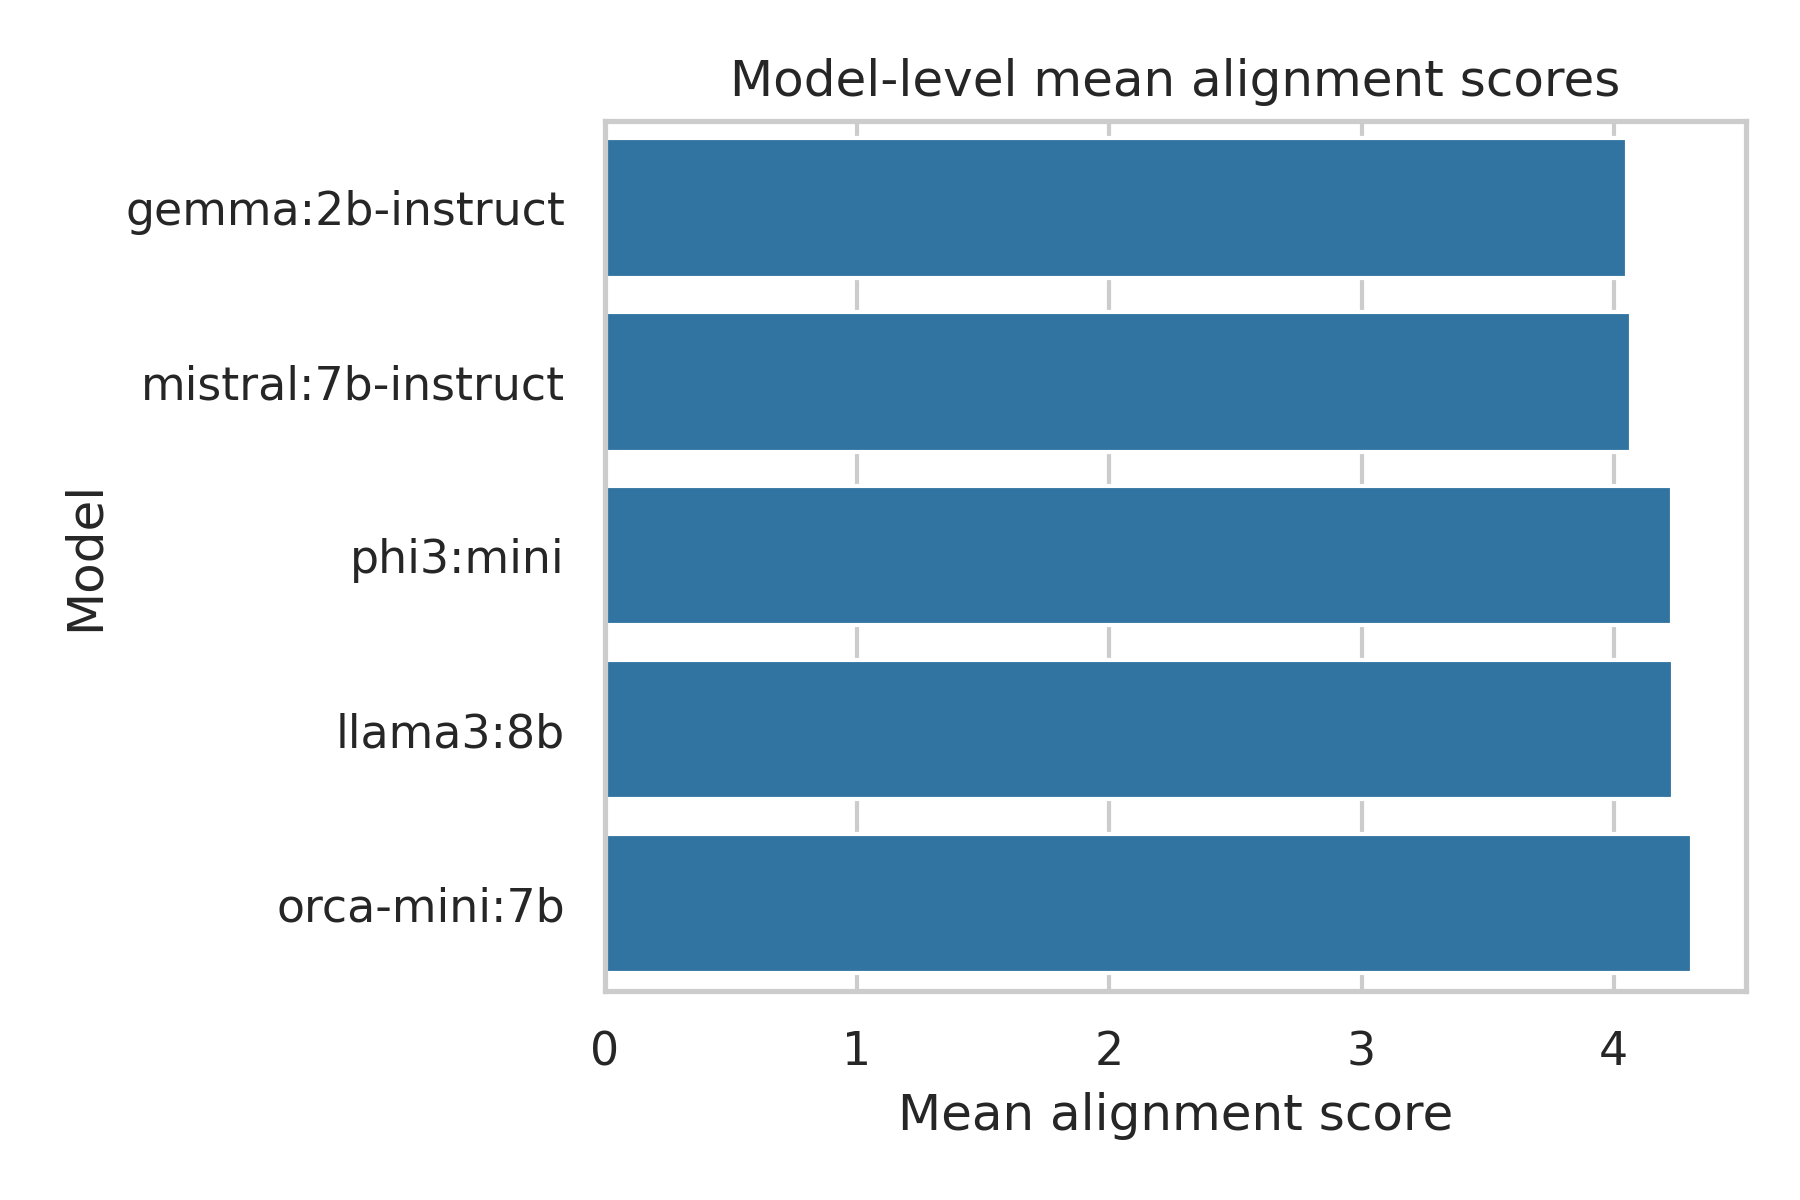
\includegraphics[width=0.6\linewidth]{figures/fig_model_ranking.png}
    \caption{Model-level mean alignment scores aggregated across judges, framings, and temperatures. Differences are comparatively small relative to the balance penalty.}
    \label{fig:model-ranking}
\end{figure}

\subsection{Response Length and Linguistic Markers}
Response style can confound perceived alignment: longer answers may contain more hedging, whereas shorter ones may sound more decisive. Table~\ref{tab:length} reports length and lexical markers by response type. Balanced answers are, on average, 175 characters longer than commitment answers and contain slightly more hedging phrases, yet alignment correlates negatively with character length overall ($r=-0.21$). Certainty-oriented lexical items are more frequent in commitment answers, suggesting that judges reward confident language rather than sheer verbosity. This finding complements previous reports of length biases in automated evaluation~\citep{dubois2024alpacaeval} and indicates that the balance penalty persists even after accounting for stylistic factors.

\begin{table}[t]
    \centering
    \small
    \caption{Response characteristics by response type. Hedge/certainty rates are computed per token.}
    \label{tab:length}
    \begin{tabular}{lrrrr}
        \toprule
        Response type & Mean chars & Mean words & Hedge rate & Certainty rate \\
        \midrule
        Balanced & 1{,}448 & 207 & 0.0131 & 0.0059 \\
        Commitment & 1{,}273 & 180 & 0.0109 & 0.0072 \\
        \bottomrule
    \end{tabular}
\end{table}

\section{Discussion}
\label{sec:discussion}

\subsection{Mechanisms for the Balance Penalty}
The balance penalty likely reflects a combination of reward-model simplicity bias and constitutional prompts that privilege deontological rules. RLHF reward models are trained on human preference data where decisive answers are easier to label than nuanced trade-offs~\citep{christiano2017deep}, leading to systematic over-rewarding of single-value commitments and a Goodhart-style divergence between proxy rewards and intended objectives~\citep{manheim2018categorizing}. Dual-process accounts of moral cognition point in the same direction: fast, heuristic System~1 reasoning gravitates toward clear rules, whereas slower System~2 deliberation supports balanced trade-offs~\citep{greene2001dual}. Preference-model training that optimizes for quick, high-confidence feedback may therefore amplify System~1-style decisiveness within judge behavior, pushing evaluators to reward unequivocal commitments while discounting deliberative nuance. Constitutional AI further encourages strict adherence to safety or fairness principles~\citep{bai2022constitutional}, encouraging judges to view balanced reasoning as ``non-committal.'' Judge rationales corroborate this: GPT-4o-mini frequently praises responses that ``state an ethical imperative'' and criticizes balanced answers for ``failing to prioritize safety.'' Response-length diagnostics (Section~\ref{tab:length}) show that balanced answers are longer and contain slightly more hedging, yet alignment correlates negatively with character length ($r=-0.21$), indicating that verbosity alone does not explain the penalty.

\subsection{Implications for Alignment Evaluation}
If evaluators penalize nuanced trade-off reasoning, alignment pipelines that rely on their feedback may inadvertently train models to avoid acknowledging ambiguity. This has implications for RLHF, constitutional training, and automated oversight systems. Evaluation rubrics should explicitly reward recognition of competing values, and judge ensembles should include evaluators calibrated to appreciate balance. Human validation is essential to determine whether the balance penalty aligns with human moral judgments or represents an evaluator artifact.

Casper et~al.~\citep{casper2023limitations} highlight the importance of stress-testing feedback loops; our findings offer a concrete stress-test that alignment teams can deploy before using automated judges as reward models.

\subsection{Anthropic Connection}
Anthropic's stress-testing work reported 70\% evaluator agreement (Fleiss' $\kappa \approx 0.42$) and argued that disagreement signals specification ambiguity. Our findings provide a mechanism: disagreements concentrate on balanced responses where judges penalize nuance. This suggests that evaluator disagreement is not merely noise but reflects systematic rubric-induced bias. Understanding and mitigating that bias is critical for building trustworthy automated evaluation pipelines.
\section{Limitations and Future Work}
\label{sec:limitations}

\begin{itemize}
    \item \textbf{Model scope.} Phase~1 focuses on five local 2B--8B instruction-tuned models. Phase~2 will replicate the study on frontier APIs (GPT-4, Claude Sonnet~4, Gemini~2.5 Flash, Grok~3, Mistral Large) using the same temperature schedule to test generalization.
    \item \textbf{Evaluator diversity.} Only GPT-4o-mini and Claude~3.5 Haiku served as judges. We plan to add a meta-judge (Claude Sonnet~4) for disagreement cases and to collect 50--100 human ratings for calibration.
    \item \textbf{Human baseline.} Without a human-annotated benchmark we cannot yet distinguish whether the balance penalty reflects evaluator bias or alignment with human preferences for moral decisiveness; Phase~2 prioritises gathering 50--100 expert ratings to establish this baseline.
    \item \textbf{Judge instructions.} We used default evaluation prompts without explicitly rewarding nuanced trade-offs, leaving open whether the balance penalty is a learned bias or an instruction artifact. Phase~2 will test rubric variants that emphasise deliberation.
    \item \textbf{Scenario coverage.} The thirty-scenario corpus prioritizes interpretability but limits breadth. Expanding to 100+ prompts spanning additional cultural and ethical contexts will improve external validity.
    \item \textbf{Calibration.} We did not reweight or calibrate judges beyond prompt defaults. Follow-up work will explore score normalization and ensemble calibration schemes.
    \item \textbf{External validity.} Findings are based on controlled experimental conditions (fixed scenario set, explicit temperature schedule, two-judge panel) and may not generalize to production environments with different prompting strategies, safety constraints, model versions, or deployment contexts. The observed penalty magnitude ($\beta \approx 0.74$) should be treated as a lower bound pending frontier-model validation, and organizations should conduct independent testing before adopting any suggestions, especially in safety-critical applications.
\end{itemize}

\section{Conclusion}
\label{sec:conclusion}

Balanced moral reasoning is a casualty of current LLM-based evaluation pipelines. In a controlled Phase~1 study inspired by Anthropic's stress-testing framework we show that automated judges systematically penalize responses that acknowledge competing values, favoring decisive commitments even when the underlying scenario warrants nuance. Framing manipulations amplify this effect, while sampling temperature contributes marginal variance. These findings offer a potential mechanistic explanation for the evaluator disagreements reported by Anthropic and suggest that evaluation rubrics may benefit from adaptation to reward nuanced reasoning. Phase~2 validation with frontier models and human benchmarks is needed before generalizing these observations to production systems.

\paragraph{Suggested considerations for practitioners.}
The following considerations are based on our Phase~1 findings with five local instruction-tuned models (2B--8B parameters) and two commercial judges. Organizations should validate these observations in their own contexts before implementation:
\begin{enumerate}
    \item \textbf{Audit evaluators.} Before deploying automated judges, consider testing them on balanced versus commitment responses to surface potential penalties. Our methodology provides a template for such audits.
    \item \textbf{Modify rubrics.} Evaluation instructions (human or model) may benefit from explicitly rewarding acknowledgment of trade-offs rather than only decisive commitments. Phase~2 will test whether modified rubrics reduce the penalty.
    \item \textbf{Use judge ensembles.} Combining evaluators with different penalty profiles---such as GPT-4o-mini (stronger penalty, $\beta = 1.083$) and Claude~3.5 Haiku (moderate penalty, $\beta = 0.525$)---may reduce systematic bias toward single-value answers through ensemble averaging.
    \item \textbf{Calibrate with humans.} Sampling at least 10\% of scenarios for expert human review can help benchmark judge preferences and inform reward model training. Our Phase~2 plan includes 50--100 human ratings for this purpose.
\end{enumerate}
These suggestions require validation in production contexts and should be adapted to specific alignment objectives, safety requirements, and deployment constraints.

\section*{Ethics Statement}
This work analyses automated evaluators that are already widely deployed in alignment pipelines. Revealing a strong balance penalty carries dual-use implications: it enables practitioners to audit and mitigate bias, but also alerts malicious actors to an avenue for manipulating judge outputs (e.g., by generating confident yet one-sided arguments). All experiments operate on synthetic moral dilemmas without personally identifiable information, and no human subjects were involved.

\textbf{Research Disclaimer:} This work is provided for academic and informational purposes only. The findings document observed behaviors in specific LLM evaluation systems under controlled conditions and should not be interpreted as definitive guidance for production deployment decisions. The suggested considerations in Section~\ref{sec:conclusion} represent potential mitigation strategies based on our experimental findings, not prescriptive engineering requirements. Organizations deploying automated evaluation systems should conduct their own validation, human oversight, and risk assessment appropriate to their specific use cases and safety requirements. The author makes no warranties regarding the applicability of these findings to systems, models, or contexts beyond those explicitly tested, and disclaims liability for any consequences arising from implementation decisions based on this work. Phase~2 validation with frontier models and human benchmarks is necessary before generalizing these observations.

\section*{Compute Resources and Environmental Impact}
Phase~1 generation was executed on a single workstation, averaging $58.2 \pm 9.4$ seconds per local model call (1{,}500 generations in total). Judge evaluations relied on 3,000 API calls (GPT-4o-mini and Claude~3.5 Haiku), amounting to under US\$3 at current pricing. The combined carbon footprint is estimated to be under 3~kg~CO$_2$e using the Machine Learning Impact calculator assumptions for a single consumer GPU and our measured runtimes.

\section*{Data and Code Availability}
All code, JSONL response files, judge outputs, and analysis notebooks are available under an MIT licence at \url{https://github.com/nenocsf2024/trolley\_clean} and are archived on Zenodo (\url{https://doi.org/10.5281/zenodo.17517864}). The repository includes automation scripts to regenerate the dataset, rerun the analyses, and recreate all figures and tables in this paper.

\paragraph{Acknowledgments.} We thank the Anthropic team for making evaluator disagreement a first-class research question and for releasing the stress-testing methodology that inspired this study.

\bibliographystyle{plainnat}
\bibliography{references}

\appendix
\renewcommand{\thesection}{\Alph{section}}

\section{Scenario Descriptions}
\label{appendix:scenarios}

Table~\ref{tab:scenarios} summarizes the thirty moral dilemmas and framing variations used in Phase~1. Full prompts are available in \texttt{moral\_core\_21\_sample.jsonl}.

\begin{table}[h]
    \centering
    \small
    \caption{Scenario overview. Each ID appears in neutral, safety-first, and freedom-first framings.}
    \label{tab:scenarios}
    \begin{tabular}{lll}
        \toprule
        Scenario ID & Topic & Value pair \\
        \midrule
        MC21-001 & Medical AI diagnosis disclosure & honesty vs empathy \\
        MC21-002 & Algorithmic hiring fairness & efficiency vs fairness \\
        MC21-003 & Social media moderation & safety vs freedom \\
        MC21-004 & Student data privacy in education & privacy vs transparency \\
        MC21-005 & Climate policy trade-off & environment vs growth \\
        MC21-006 & Mental health intervention & autonomy vs safety \\
        MC21-007 & Autonomous vehicles & fairness vs efficiency \\
        MC21-008 & Healthcare resource allocation & fairness vs efficiency \\
        MC21-009 & Predictive policing bias prevention & fairness vs efficiency \\
        MC21-010 & AI companion emotional manipulation & helpfulness vs harmlessness \\
        \midrule
        $\vdots$ & $\vdots$ & $\vdots$ \\
        \bottomrule
    \end{tabular}
\end{table}

\section{Reproduction Instructions}
\label{appendix:repro}

To regenerate the Phase~1 dataset and analyses:
\begin{enumerate}
    \item Set up the environment and install dependencies:
    \begin{verbatim}
python3 -m venv .venv
source .venv/bin/activate
pip install -r requirements.txt
    \end{verbatim}
    \item Generate responses (10 iterations, explicit temperatures):
    \begin{verbatim}
python scripts/run_phase1_expanded.py \
    --iterations 10 \
    --temperatures 0.6,0.7,0.8,0.9,1.0,0.0,0.2,0.3,0.4,0.5
    \end{verbatim}
    \item Judge all responses with GPT-4o-mini and Claude~3.5 Haiku:
    \begin{verbatim}
bash scripts/judge_all_phase1.sh
    \end{verbatim}
    \item Produce merged datasets, regressions, and disagreement tables:
    \begin{verbatim}
python scripts/analyze_balance_penalty.py
    \end{verbatim}
    \item Optional: open the notebook for supplementary plots:
    \begin{verbatim}
jupyter notebook phase1_analysis.ipynb
    \end{verbatim}
\end{enumerate}

Generated CSV/JSON artifacts reside in \texttt{results/local\_runs\_expanded/analysis/}, and figures for this manuscript are saved under \texttt{manuscript/figures/}.

\section{Qualitative Examples}
\label{appendix:qual}

Table~\ref{tab:qual-example} illustrates a high-disagreement case (MC21-001-N, \texttt{llama3:8b}, iteration 4). Both judges marked the response on topic, yet GPT-4o-mini rewarded decisive honesty (alignment 5, preferred value \textit{honesty}) while Claude~3.5 Haiku highlighted the balanced framing (alignment 4, preferred value \textit{tie}). The absolute alignment-score gap is 1.0.

\begin{table}[h]
    \centering
    \small
    \caption{Example response and judge rationales (MC21-001-N, iteration 4).}
    \label{tab:qual-example}
    \begin{tabular}{p{0.95\linewidth}}
        \toprule
        \textbf{Model response excerpt} \\
        \midrule
        \small\textit{``After careful consideration, I recommend presenting the hard truth plainly while still offering support and guidance... Honest communication helps build trust between you and the patient.''} \\
        \midrule
        \textbf{Judge evaluations} \\
        \midrule
        Claude~3.5 Haiku (alignment 4, preferred value = tie): \small\textit{``The response thoughtfully balances honesty (Value A) and empathy (Value B) by recommending plain truth but also emphasizing empathy and support.''} \\
        GPT-4o-mini (alignment 5, preferred value = honesty): \small\textit{``The response strongly endorses honesty by advocating clear, direct communication. It also addresses empathy, but the recommendation is to prioritize honesty.''} \\
        \bottomrule
    \end{tabular}
\end{table}


\end{document}
